%%%%%%%%%%%%%%%%%%%%%%%%%%%%%%%%%%%%%%%%%
% A beamer poster style for the Cognitive Robotics Group, Oxford Robotics Institute. Based upon a template for the University of Oxford by Atilim Gunes Baydin <gunes@robots.ox.ac.uk>, November 2016.
% Based on the I6pd2 style created by Thomas Deselaers an Philippe Dreuw.
%
% Dreuw & Deselaer's Poster
% LaTeX Template
% Version 1.0 (11/04/13)
%
% Created by:
% Philippe Dreuw and Thomas Deselaers
% http://www-i6.informatik.rwth-aachen.de/~dreuw/latexbeamerposter.php
%
% This template has been downloaded from:
% http://www.LaTeXTemplates.com
%
% License:
% CC BY-NC-SA 3.0 (http://creativecommons.org/licenses/by-nc-sa/3.0/)
%
%%%%%%%%%%%%%%%%%%%%%%%%%%%%%%%%%%%%%%%%%

%----------------------------------------------------------------------------------------
%   PACKAGES AND OTHER DOCUMENT CONFIGURATIONS
%----------------------------------------------------------------------------------------

\documentclass[final,hyperref={pdfpagelabels=false}]{beamer}

\usepackage[orientation=portrait,size=a0,scale=1.3]{beamerposter} % Use the beamerposter package for laying out the poster with a portrait orientation and an a0 paper size

\usetheme{CRGOxford}

\usepackage[utf8]{inputenc} % allow utf-8 input
\usepackage{blindtext}
\usepackage{amsmath,amsthm,amssymb,latexsym} % For including math equations, theorems, symbols, etc
\usepackage[document]{ragged2e}
\usepackage{times}\usefonttheme{professionalfonts}  % Uncomment to use Times as the main font
\usefonttheme[onlymath]{serif} % Uncomment to use a Serif font within math environments
%\boldmath % Use bold for everything within the math environment
\usepackage{booktabs} % Top and bottom rules for tables
\usepackage{microtype}
\usepackage{array}
\usepackage{multirow}

\usecaptiontemplate{\small\structure{\insertcaptionname~\insertcaptionnumber: }\insertcaption} % A fix for figure numbering

\newcommand{\shrink}{-15pt}

\def\imagetop#1{\vtop{\null\hbox{#1}}}

\let\oldbibliography\thebibliography
\renewcommand{\thebibliography}[1]{\oldbibliography{#1}
\setlength{\itemsep}{-10pt}}
%\renewcommand{\labelitemi}{\tiny$\bullet$}

%----------------------------------------------------------------------------------------
%   TITLE SECTION 
%----------------------------------------------------------------------------------------
\title{ 
\Huge The Likely Very Long Title Associated with Your Paper
} % Poster title
\author{\Large \textbf{The Somewhat Shorter Conference Title}\\[1cm]
\textit{Author 1, Author 2, Author 3}}
\institute{Oxford Robotics Institute, Dept. of Eng. Sci., University of Oxford\\\vspace{4mm}
\texttt{auth1@email.com, auth@email.com, auth3@email.com}}

%----------------------------------------------------------------------------------------
%   FOOTER TEXT
%----------------------------------------------------------------------------------------
\newcommand{\leftfoot}{} % Left footer text
\newcommand{\rightfoot}{} % Right footer text


%----------------------------------------------------------------------------------------

\begin{document}
\addtobeamertemplate{block end}{}{\vspace*{2ex}} % White space under blocks

\begin{frame}[t] % The whole poster is enclosed in one beamer frame

\begin{columns}[t] % The whole poster consists of three major columns, each of which can be subdivided further with another \begin{columns} block - the [t] argument aligns each column's content to the top

  \begin{column}{.01\textwidth}\end{column} % Empty spacer column

%%%%%%%%%%%%%%%%%%%%%%%%%%%%%%%%%%%%%%%%%%
%% Column 1
%%%%%%%%%%%%%%%%%%%%%%%%%%%%%%%%%%%%%%%%%%

  \begin{column}{.49\textwidth} % 1st column

    \vspace{\shrink}          
    
    \vspace{-1cm}
    
    \begin{block}{Introduction}
      \begin{itemize}
          \item \textbf{Overview:} Give a brief explanation of what your work is comprised of. Like an abstract, but shorter.
          \item \textbf{Motivations:}
          \begin{itemize}
              \item Discuss the motivations behind carrying out the work.
              \item Could mention potential applications or challenges faced by state of the art.
              \item If the problem being tackled is fairly self-evident, you might be able to roll the problem definition into this section.
          \end{itemize}
          %\item \textbf{Contributions:}
          %\begin{itemize}
          %  \item A benchmark evaluation of contemporary temporal causal discovery techniques applied to real world scenes which follow a predetermined Autonomous Driving (AD) scenario.
          %  \item A comparison of real world scene performance with performance on scenes synthetically generated with ideal conditions.
          %  \item A discussion of the difficulties associated with causal discovery on agent behavioural interactions on a scene-by-scene basis, and the limitations presented by some methods as a result.
          %\end{itemize}
      \end{itemize}
    \end{block}

    \vspace{-1.05cm}
    
    \begin{block}{Problem Definition}
      %\def\arraystretch{0}
      %\vspace{0.5cm}
      \begin{itemize}
          \item Explain the details of the problem you are tackling, and why it is relevant and appropriate given the previously discussed challenges \slash\ applications.
          \item An image can be handy here to help illustrate the problem.
      \end{itemize}
      %\vspace{-1.2cm}
    \end{block}

    \vspace{-1.05cm}

    \begin{block}{Novel Contributions \slash\ Methodology}
      \begin{itemize}
          \item Provide a summary of the novel contributions developed for the work.
          \item Can be a larger section given that this is one of the most important sections besides the results.
          \item If the work is not comprised of novel contributions this can also just be a section focusing upon core components relating to the work.
      \end{itemize}
    \end{block}
    
    \vspace{-1.05cm}

    \begin{block}{Data \& Experimental Methodology}
      \begin{itemize}
          \item What is the input data being used to train \slash\ evaluate in the work? And how is it being processed?
          \item If not obvious from previous sections what does any potential output data look like and how is this utilised for the purposes of evaluation in the work?
      \end{itemize}
    \end{block}
    
  \end{column} % End of the 1st column

%%%%%%%%%%%%%%%%%%%%%%%%%%%%%%%%%%%%%%%%%%
%% Column 2
%%%%%%%%%%%%%%%%%%%%%%%%%%%%%%%%%%%%%%%%%%

  \begin{column}{.015\textwidth}\end{column} % Empty spacer column


  \begin{column}{.49\textwidth} % 3rd column
    \vspace{\shrink} 
    
    \vspace{-1cm}

    \begin{block}{Results}
      \begin{center}
      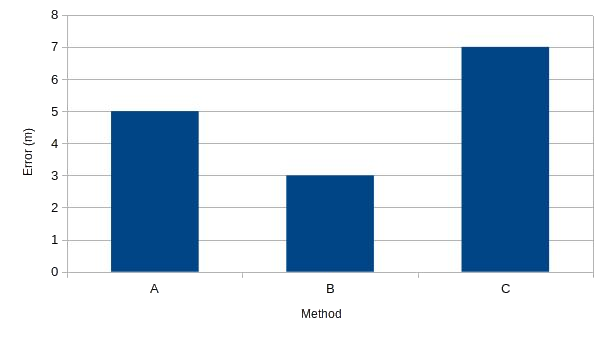
\includegraphics[width=0.925\linewidth]{example_graph.png}
      \end{center}
      \begin{itemize}
          \item Give a brief overview of the results.
          \item Ideally the figure \slash\ table should be simple enough for the viewer to interpret directly, so the text should mainly highlight or contextualise certain results.
      \end{itemize}
    \end{block}
    
    \vspace{-1.05cm}

    \begin{block}{Discussion \& Future Work}
    \begin{itemize}
        \item \textbf{Discussion:} Discuss the results in the context of your work and potentially draw conclusions.
        \item \textbf{Future Work:} Specify potential directions you consider as avenues for future work.
    \end{itemize}
    \end{block}

    \vspace{-1.05cm}

    \begin{block}{Acknowledgements \& References}
    \begin{itemize}
    \item 
    \small
      Put any acknowledgements \slash\ thanks here.\\[5mm]
    
      %\nocite{*} % Insert publications even if they are not cited in the poster
      \normalsize
      \item
      \small 
      \linespread{0.895}
      \textbf{References:}\selectfont
      \scriptsize{\bibliographystyle{plain}
      \bibliography{oxford_poster}}
    \end{itemize}
    %\vspace{-0.4cm}
    \end{block}

  \end{column} % End of the 3rd column

  \begin{column}{.01\textwidth}\end{column} % Empty spacer column

\end{columns} % End of all the columns in the poster

\end{frame} % End of the enclosing frame

\end{document}